\section{Kilath 4.1.7}
The system is modeled as 
\begin{align*}
    \dot x(t) &= v(t), \quad \dot v(t) = -\omega_0^2\,x(t), & y(t)&= v(t), & x(t_0) &= 0, \quad v(t_0) = 10.
\end{align*}
\begin{align*}
    A &= \begin{pmatrix}
        0 & 1 \\ -\omega_0^2 & 0
    \end{pmatrix} \quad C = \begin{pmatrix}
        0 & 1
    \end{pmatrix}
\end{align*}
The closed-loop observer poles are at $\omega_0$, i.e., 
\begin{align*}
    \alpha_\mathcal{O}(s) &= \left(s + \omega_0\right)\,\left(s + \omega_0\right) = s^2 + 2\,\omega_0\,s + \omega_0^2
\end{align*}
Also, 
\begin{align*}
    \alpha_\mathcal{O}(s) = \text{det}\left(SI - A + K\,C\right) &= \det\left[\begin{pmatrix}
        s & 0 \\ 0 & s
    \end{pmatrix} - \begin{pmatrix}
        0 & 1 \\ -\omega_0^2 & 0
    \end{pmatrix} + \begin{pmatrix}
        k_1 \\ k_2
    \end{pmatrix}\,\begin{pmatrix}
        0 & 1
    \end{pmatrix}\right] \\
    &= \det\left[\begin{pmatrix}
        s & -1 \\ \omega_0^2 & s
    \end{pmatrix} + \begin{pmatrix}
        0 & k_1 \\ 0 & k_2
    \end{pmatrix}\right] = \det\left[\begin{pmatrix}
        s & k_1-1 \\ \omega_0^2 & s + k_2
    \end{pmatrix}\right] \\
    &= s\,\left(s + k_2\right) - \omega_0^2\,\left(k_1 - 1\right) = s^2 + s\,k_2 + \omega_0^2\,\left(1 - k_1\right)
\end{align*}
Therefore,
\begin{align*}
    K = \begin{pmatrix}
        k_1 \\ k_2
    \end{pmatrix} = \begin{pmatrix}
        0 \\ 2\omega_0
    \end{pmatrix}
\end{align*}
The solution to the ODE is 
\begin{align*}
    x(t) &= 10\,\sin(\omega_o\,t), & v(t) &= 10\,\cos(\omega_o\,t).
\end{align*}
The simulation results for $\omega_0 = 10$\,rad/s are presented in the figure:

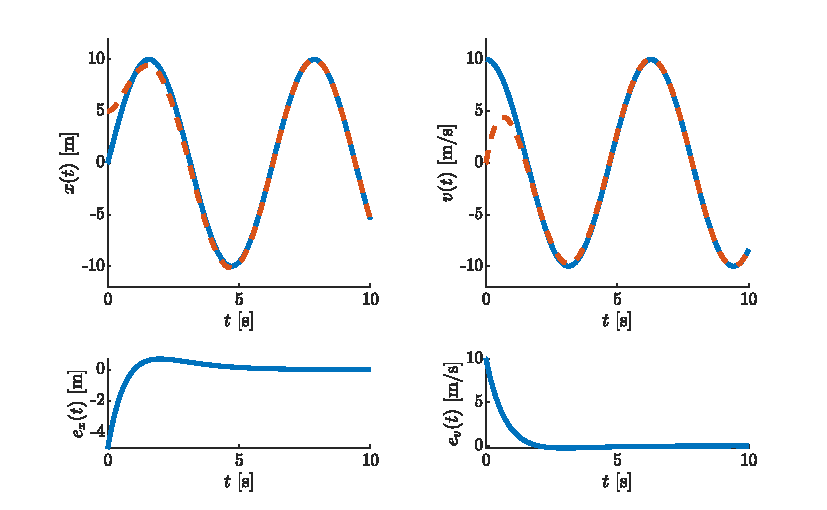
\includegraphics{figures/ex417.pdf}

The solid line is the true state and the dashed line is the estimate from the observer. 

The error dynamics are 
\begin{align*}
    \dot e &= \left(A - K\,C\right)\,e = \left(\begin{pmatrix}
        0 & 1 \\ -\omega_0 & 0
    \end{pmatrix} - \begin{pmatrix}
        k_1 \\ k_2
    \end{pmatrix}\,\begin{pmatrix}
        0 & 1
    \end{pmatrix}\right)\,e = \begin{pmatrix}
        0 & 1 - k_1 \\ -\omega_0^2 & -k_2
    \end{pmatrix}\,e,\\
    \dot e_x &= (1 - k_1)\,e_v \quad \dot e_v = -\omega_0^2\,e_x - k_2\,e_v \quad \implies \dot e_x = e_v \quad \dot e_v = -\omega_0^2\,e_x - 2\,\omega_0\,e_v.
\end{align*}
Therefore, the error will converge with a time constant of $1/\omega_0$.

\clearpage
\subsection*{Code}

\begin{matlabcode}
    clear; 
    
    omega = 1;
    v0 = 10;
    
    % system true states
    x = @(t) 10*sin(omega*t);
    v = @(t) 10*cos(omega*t);
    
    A = [0 1; -omega^2 0];
    C = [0 1];
    
    y0 = [5; 0];
    tspan = [0 10];
    [t,y] = ode45(@(t,y) observ(y,v(t),C,A,omega),tspan, y0);
    
\end{matlabcode}

\matlabheading{functions}
    
\begin{matlabcode}
    function xdot = observ(x,y,C,A,omega)
    
    K = [0; 2*omega];
    
    xdot = A*x + K*(y - C*x);
    
    end
\end{matlabcode}